\section{Discussion And Applications}
\subsection{PAS Domain - Binding Specificity}
\subsection{Elongin C - VHL Interaction}
% Subsection Introduction
In this section, we demonstrate the utility of HomologyRing to quickly give structral insight to a particular protein family and the complexes it forms. 
Study of interactions contributiong to the formation of protien complexes is done by considering the inter-chain interactions with in a hRIN. 
The inter-chain interactions are edges that connect a node representing a family of residues, here reffered to as `residue nodes', to nodes that represent an entire entity or protein chain other than the homologs identified through the BLAST search, identified here as `chain nodes'.
We will use the interactions formed by the RNA Transcription Factor B complex, to demonstrate these capabilities. 

Transcription Factor B, also known as SIII or simply Elongin, is a protein complex responsible for promoting RNA polymerase II elogation by suppressing the function of arresting sites within a transcription window \cite{Chen2023}. In this sense it has been identified as an elongation factor regulating transcription by RNA polymerase II. Transcription processes are most commonly thought of as being regulated by initiation factors. However, regulation of the process during elongations is increasingly understood as being significantly important. The Elongin complex is seen to be dynamic and known to have several other interacting factors affecting elongation behaivor. % https://www.nature.com/articles/s41594-023-01138-w#ref-CR8 % CUL5–RBX2 complex
We will primarially focus our discussion on ELOC: using it as a query inorder to build an hRIN with HomologyRing to observe inter-chain interactions in the Transcription Factor B (SIII) and related complexs. 
Comparing structural insites gained through HomologyRing to results from the literature will be used to demonstate the usefulness of the tool and information contained in the resulting hRINs.  

%% Move this to where we start talking about the pipeline being run
It this case, it is worth noting that we are not primarially concerned with the construction of a family of homolog proteins per se. Rather, we can expect a BLAST search of the PDB to return many ELOC orthologs, or human isoforms (of which there are three \cite{Chen2023}), resulting in a family of high sequence similarity, but may very considerably in the entities present in each complex structure. % stub
%%% END STUFF TO MOVE

%% Complex introduction
Before detailing the running of the pipeline and intrepeting the resulting hRIN, we pervide some context for the significance of Elongins structure and function. 
The SIII compex is composed of three elongins: A, B, and C and are highly conserved in Eukaryotes. 
These elongin protein products are respectively refered to by their short gene names: ELOA, ELOB, and ELOC.
Behaivor of the SIII elongation factor is well studied experimentally, and has enjoyed a lot of attention. However, much of its function on a mechanistic level is yet to be fully understood. 
% ELOA structure and function
ELOA as a monomer has been seen to promote elongation by RNA Pol II alone \cite{Aso1995}, as ELOA is the is responible for binding in the SIII Elongin complex with the larger RNA Poly II complex where Elongins B and C are regulatory subunits. Additionally, ELOB and ELOC are seen to form a subcomplex independent of ELOA. \cite{Chen2023}, and as will be seen later, is under represented in structures of complexes in the PDB containing ELOC. 
As a result, we will primarially discuss the interaction between ELOC and ELOB. 
% ELOB structure and function
ELOB (seen in \ref{fig:SIII-structure}), 
Ubiquitin-like protein %https://www.nature.com/articles/s41594-023-01138-w#ref-CR14
% Globular core
% Disordered tail at X-terminus
% ELOC structure and function
SCF ubiquitin ligase subunit Skp1 % ??? I think this is describing a different complex
% https://www.nature.com/articles/s41594-023-01138-w#ref-CR8
Seen to promote the activity of ELOA %https://www.nature.com/articles/s41594-023-01138-w#ref-CR14

Figure \ref{fig:SIII-structure} shows an ELOB - ELOC complex interacting with a portion of pVHL.

We show a complex of ELOB, ELOC, pVHL incomplex with a region of HIF in Figure \ref{fig:SIII-structure}.
\begin{figure}[ht] % replace with [H} if position is causing problems.
    \centering
    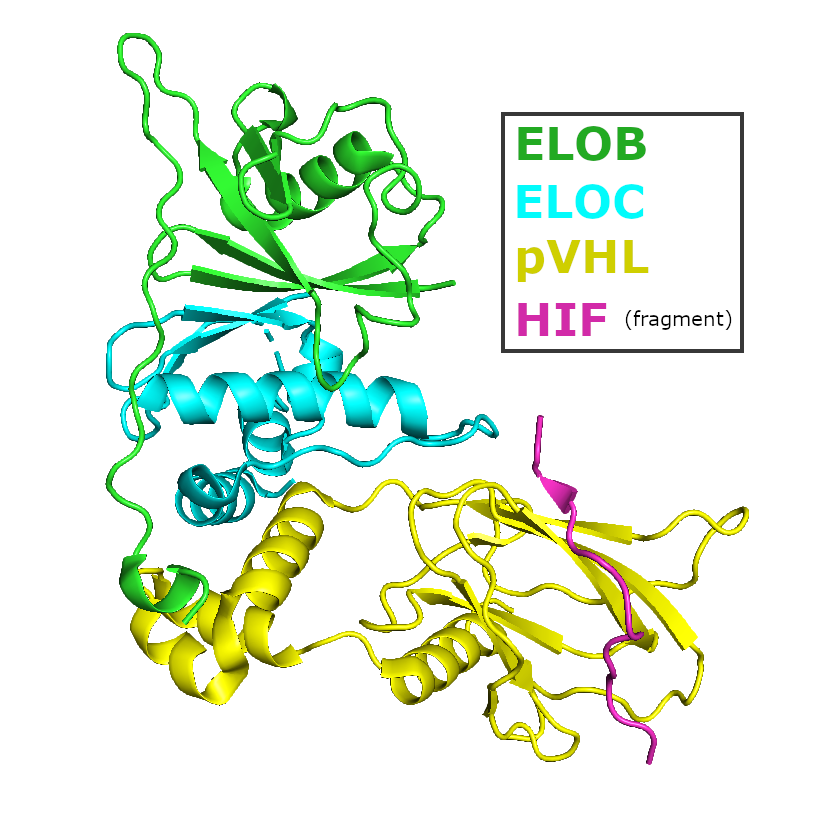
\includegraphics[width=0.5\textwidth]{fig/SIII_1LM8.png}
    \caption{PDB: 1LM8; Complex of Elongin B,C with pVHL and HIF-region \cite{Min2002}.}
    \label{fig:SIII-structure}
\end{figure}

% Introduce pVHL

Notabale regulation activity comes from the SIII interaction with the Von Hippoel-Lindau Tumor Suppressor Protein (pVHL) which is coded for by the VHL gene. Elongins B and C have are known to interact with pVHL in the SIII complex. pVHL, in this interaction is seen to inhibit transcription elongation. 
%pVHL context
The pVHL product is well-known a regulator of many different pathways and known to interact with several other proteins \cite{Tabaro2016}. However, the protein has recieved much attention for its role as a tumor suppressor \cite{}, and owes its name for its associated Von Hippel Lindau syndrome -- an inheritable genetic mutation to the VHL gene which is associated with a very high propensity for tumor devlopment in many highly vascularized tissues throughout the body. 

At the protein level, VHL is known for its role in regulating tissue response to hypoxic, or low oxygen, conditons. 
Spesifically, pVHL is seen to be contribute the the ubiquitination of hypoxia-inducible factors (HIFs). 
HIFs are transcription factors, or proteins that bind to spesific regions of DNA to regulate their transcription.
They are a key component the process through wich mamilian cells respond to hypoxic conditons, or prolonged leveles of low oxygen. 
Hypoxia is highly relevant to many forms of cancer, as tumos growing and eventually cutting themselvs off from blood supply in their interior are a common pattern. HIF, working as a transcription factors, can promote the thranscription of various different genes which may serve to mitigate the effects of hypoxia, correct it, or signal for the destruction of the cell. One known mechanism for addressing the issue of hypoxia in tissue is signialing for the additional vasculature, thus increasing the supply of blood and oxygen to the area. This behaivor is highly characteristic of the tumors seen in VHL syndrome, occuring in highly vascularized areas such as parts of the brain, retina, and spine, among others. % https://en.wikipedia.org/wiki/Von_Hippel%E2%80%93Lindau_tumor_suppressor#cite_note-Ben-SkowronekKozaczuk2015-5

%pVHL structure

% funtion , types of mutations to VHL
Healty pVHL, in complex with ELOB and ELOC,  tags HIFs with Ubiquitin, signiling for their destrction, and thus working to down regulate a tissues hypoxia response. Mutations to the protein such as the ones seen in VHL syndrome



%%% pVHL HIF interaction, structure
HIF contains a highly conserved proline containg region which is the binding substrate where the HIF will bind to pVHL. 
In hypoxic enviroments, the prolines in this region will experice hydroxulation, a post translational modification where proline will gain an hydroxyl groub on the sidechains gamma carbon. This modification enables pVHL-HIF interactions and subsequent ubiquinition of HIF, a process that eventually leads to the destruction of the HIF, freeing the gene region to which it was previously bound. This process is critical for allowing cells to variably express genes based on the amound of oxygen avaible to the cell, allowing for behaivoral changes that allow for its survival like angiogenisis or alternatively programmed cell death in low oxygen senerios \cite{Carmeliet1998}. 

%pVHL function (breakdown)
% pVHL interaction sites

This well-studied complex has recieved much attention for its role in several cancers. 
% This should be moved somewhere else --- possibly in the section where the PDB database is introduced
% Write a shorter blurb explaining this idea to go here
It is important to note that a homology search of the PDB does not neccessarily return a set of distinct, evolutionarily related sequences. Instead, the Homology search as implemented by BLAST reutrns sequences with high sequnce similarity to the query. This will most likely many different structures for the same protein, as the PDB may contain many structures for the same protein.
This is desiarable behaivor, given that tese different enteries may correspond to the protein in different biological contexts, with differences in temprature or pH; additionally a protein of interests may form different complexes with many interactors, or experience conditional conformal variations. 
All of these factors influcence the structure and corresponding RIN of a protein. Given this networks with noteworthey differences in topology can be seen to represent the same protein chain. By coreating a hRIN for a sigle protein, we obtain a single object that may be used to represent a protein that captures both  variations and conserved features of a protein.


%PIPELINE AND RESULTS
The preceding sub-sections serve to illustrate the many complicated interactions in which ELOC participates. Each of these interactions is quite nuanced, and a complete picture of all possible interactions and their functioning at a molecular level is a very time consuming process to come to understand. Furthermore, in this case there is still much that remains not compleatly understood. Here we will utilize HomologyRing to quickly an object capturing structural information about protein-protein interactions at the residue level. This may be used as an overview, providing researchers a quick introduction to wich sites and compounds are involved in interactions in a protein family, or as a technical, well defined mathematical object, wich could be used for more quantitive analysis. In this section we will demonstrate the former, using HomologyRing to quickly gain initial insight in to the Elongin Complex.

The  section as a detailed account of the considerations commonly made when analysing hRINs; aswell as challenges presented by the data, and how tools provided by HomologyRing can adress them. Namely, the propensity and biological significance of different types of interactions, means that a filtering process can greatly aid visualization. Furthermore, variation in the protein chains present in each structure included in the family needs to be considered when conserned with the conservation of interactions.

After initiating the pipeline to build the hRIN, we will first address the different protein chains included in the set of structures. 
Since we are here concerned with interactions of multiple protein chains, we are required to restrict the use of the pipeline in this case to a homology search of the PDB, as predictions avaible in the AlphaFold Database are limited to single chain structures, preventing the study of inter-chain interactions. 
Bias in the PDB in some ways limit the usefullness of the quantitive information in the graph. The probability weights in the inter-chain edges of the graph are heavily influenced by the frequency with which published experimental structures have captured any given two entities in a single structure. As discussed, the size of the greater complex associated with Elongin is dynamic and highly variable. 
Presense of particular entities in experimental structures is also influenced by factors such as interest in particular aspects of a complex within the research community and difficulty of chrystialization. 
%Both of these factors distance the edge weight data from being effective measures of the propensity for an entities interaction in a biological context and such biases should be considered for more statistically rigorous analysis aimed at studying such interactions.

We begin our analysis of the Elongin complex by centering our focus on the ELOC chain, using it as our query structure. And with this we may begin spesifying parameters to construct a HomologyRing quert. Spesifically, the query chain is taken from the \texttt{AUTH C} chain of the PDB structure \texttt{1LM8}, which is a x-ray chrystal structure of the ELOB-ELOC dimer in complex with a fragment of pVHL \cite{Min2002}. The corresponding query sequence is 88 residues long, and maps to uniprot accention {Q15369-2} isoform, differing from the cannonical sequence by an omission of 16 residues from the N-terminal, or beginning of the sequence. 
The PDB Europe Knowledge Base lists 164 structures in the PDB mapped to the ELOC Uniprot gene: \texttt{Q15369}. However, many more close homologs exist with high sequence similarity.
Creating an hRIN win an aim to create a comprehensive account of all ELOC structures in the PDB is perfectly feasible with the RingHomology pipeline and can capture infromation from all 164 structures comprising more than 500 MB of information in a few minutes on consumer hardware. However, for the sake of simplicity of visuilization we limit the homolgy search to just 128 results here. Since in this use case we aim to perform a narrow analysis on spesifically the ELOC gene, we set a conservitive E-value theshold for the homology search of $5 \times 10^{-3}$, restricting results to sequences with high pairwise similarity to the query sequence.

Running the pipeline quickly constructs an hRIN. In this section we will use the analysis tools included in the HomologyRing package to explore the information contained in this object on a sequence, structural, and network level. Firstly, examining the amino acid sequences belonging to each homolog chain is an excellent way to begin intrepreting information about the family. The MSA created by the pipeline is used internally for the definition of nodes in the network, and its visualization serves as a useful aid for understanding the hRIN. Figure \ref{fig:eloc-msa} shows a representation of the MSA where residues in each homolog sequence is colored according to CLUSTAL colors, which groups amino acid residues according their chemical and physical properties, This is covered in more detail in \ref{sec:contact-mask} with the exception that here no contact information is displayed. \todo{Finish section detailing the MSA analysis contact plots}
As seen in the figure, this family has a high degree of sequence identiy. This is an anticipated result due to the number of ELOC enteries in the PDB and restrictive E-value set when running the pipeline. The exact identity of the protein chains are discussed shortly in this section. The MSA shows high identity in the majority of columns, with a handful of 1-2 residue deletions introducing gaps, and only a few notable substatutions. 
Residues 35 - 42 are clearly seen to have low occupancy compared to the rest of the residues. Referencing structures in the family as well as Interpro entries, show that the region correspond ot a hairpin turn of variable length. These are common regions of variation, and as we will see, correspond to a region with little significance to inter-chain interactions seen in the PDB complexes. \todo{Change if this is wrong}
The high identity in the family is useful reducing the overall complexity of the resulting hRIN, which aids in simplifying the subsequent analyses.

%% MSA Figure
\begin{figure}[h!] % replace with [H} if position is causing problems.
    \centering
    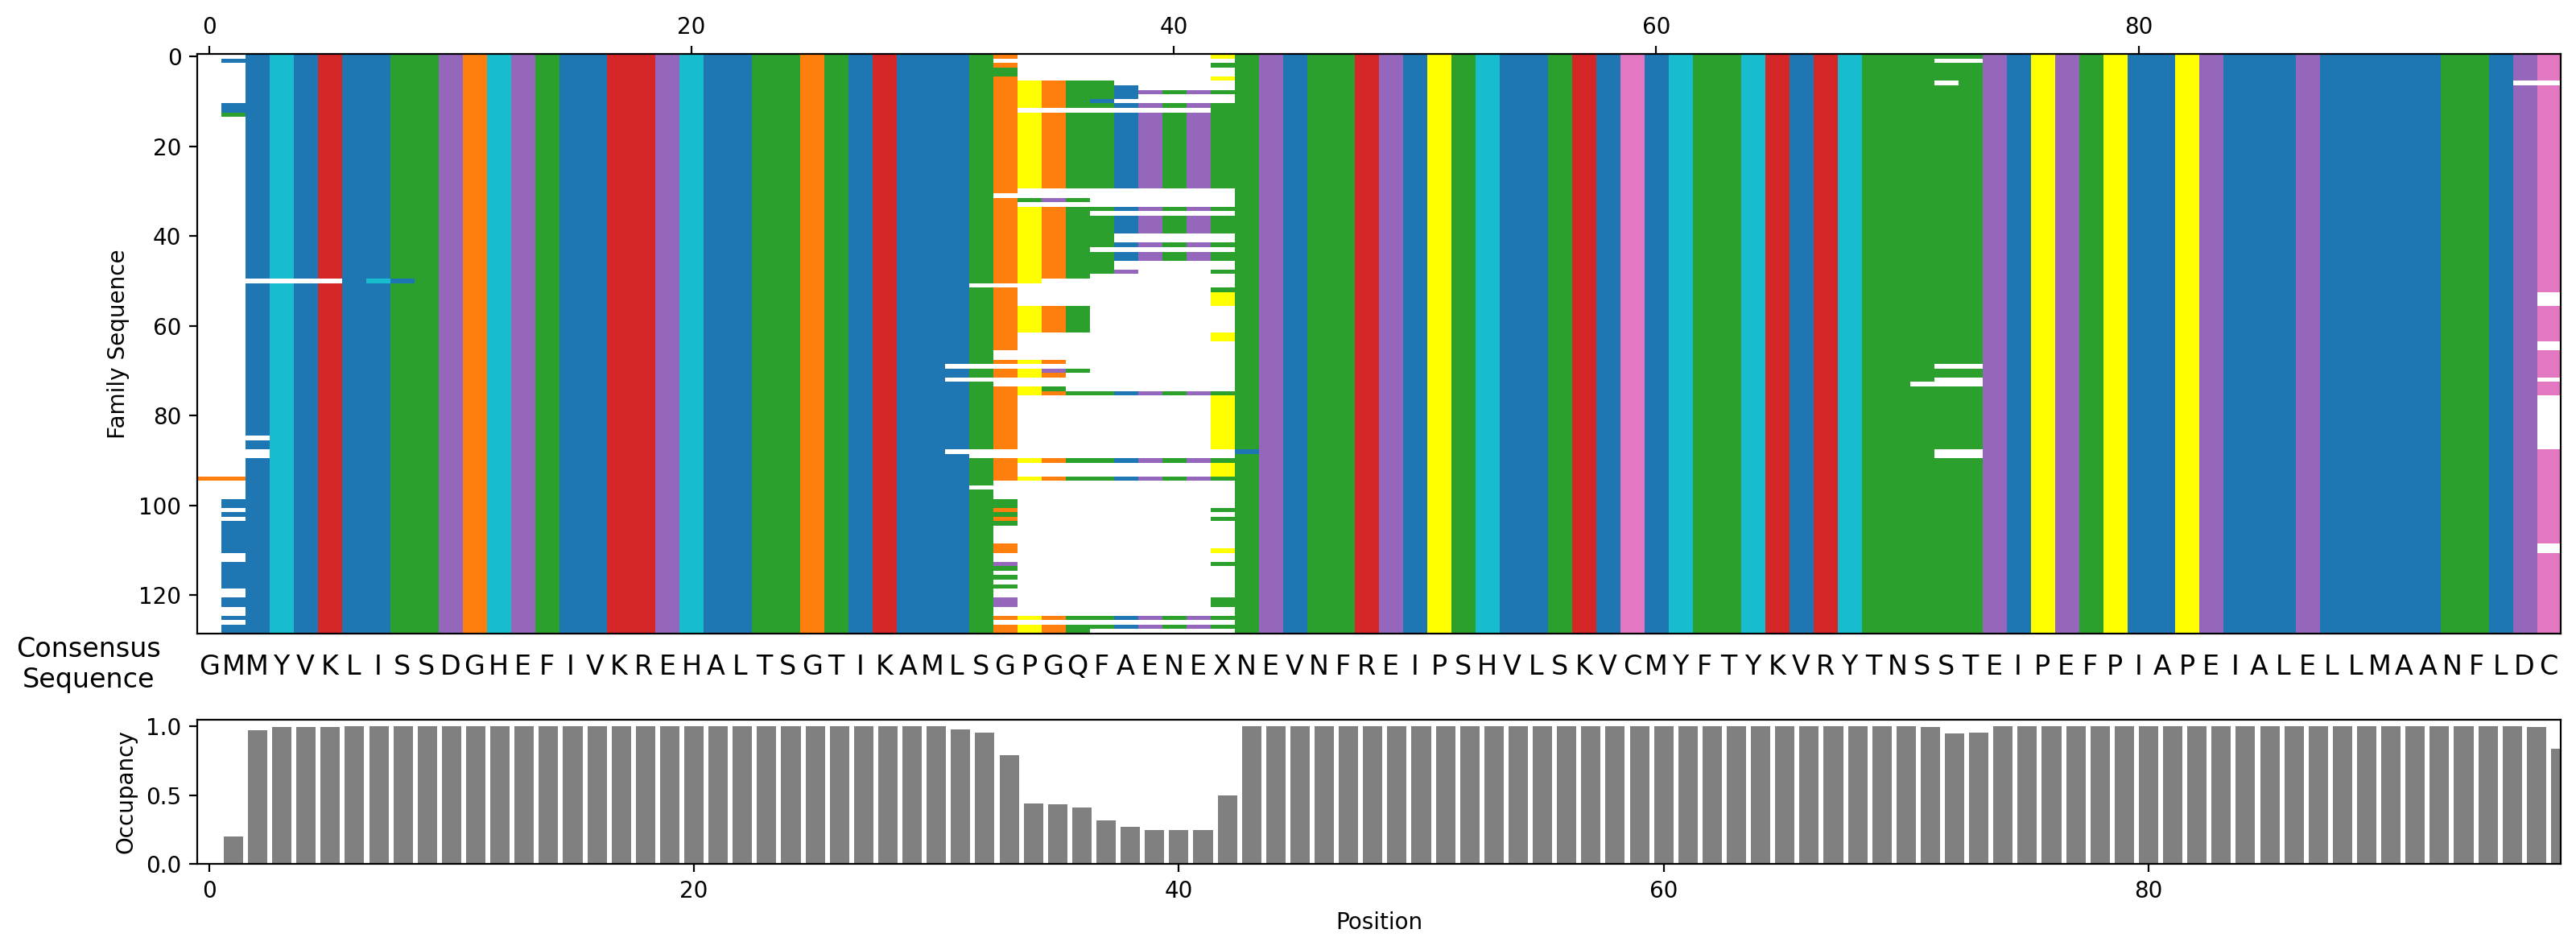
\includegraphics[width=\textwidth]{fig/ELOC-MSA.png}
    \caption{Representation of a multiple sequence alignment for the ELOC family. Created as part of the HomologyRing pipeline with Clustal$\Omega$}
    \label{fig:eloc-msa}
\end{figure}

%% Table of common protein chains
As stated, a primary aim of this analysis is structural insight into inter-chain interactions. To begin, we will summarize which protein chains are present in the families structures. This gives indication of wich proteins are commonly observed in complex with homologs of our query in the PDB and wich interactions are captured by the network. Table \ref{tab:eloc-chain-count} provides an overview of the presence of protein chains in the structure collected to form the family. HomologyRing exposes this information orginally collected from CIF metadata and includes additional information on ligand presence and are provide reference for detailed information associated with nodes in the network. 

ELOC\_HUMAN, despite being used as the query seqeunce, is only listed as present in $98.2\%$ of structures. This is due to close homologs like ELOC\_MOUSE comprising a small handful of the homolog chains included in the family.  
We also observe that the distribution of protein chain counts has a long tail. Truncated from Table \ref{tab:eloc-chain-count} was 30 different proteins that appeared in no more than 2 structures. Some are the close homologs, as previously mentioned, while others are lesser studied proteins associated with Elongin or RNA Poly II. 

\begin{table}[h!] % Use [H] for exact placement, if necessary
    \centering
    \begin{tabular}{l c c c}
    \textbf{Gene} & \textbf{Chains} & \textbf{Structures with Chain} &  \textbf{Structures with Chain (\%)} \\ \cline{1-4}
ELOB\_HUMAN & 158 & 63 & 98.4\% \\
ELOC\_HUMAN & 124 & 59 & 92.2\% \\
VHL\_HUMAN & 78 & 39 & 60.9\% \\
CUL2\_HUMAN & 38 & 18 & 28.1\% \\
RBX1\_HUMAN & 24 & 14 & 21.9\% \\
FEM1B\_HUMAN & 19 & 10 & 15.6\% \\
APBP2\_HUMAN & 16 & 5 & 7.8\% \\
PEBB\_HUMAN & 15 & 3 & 4.7\% \\
BRD4\_HUMAN & 15 & 8 & 12.5\% \\
CUL5\_HUMAN & 14 & 2 & 3.1\% \\
RASK\_HUMAN & 6 & 3 & 4.7\% \\
HIF1A\_HUMAN & 6 & 3 & 4.7\% \\
\textbf{OTHER} & 77 & 34 & 53.1\% \\
    \end{tabular}
    \caption{Number of occurences of each the most common protein chains in the family constructured by the HomolgyRing pipeline. Family consists of 129 homolog chains from 64 different unique structures from the PDB. Structures may contain more than one protein chain transcribed from the same gene. Number of structures in the family that posses the protein corresponding to the given gene are also indicated. This table serves to give an overview of wich interchain interactions are well captured within the constructed hRIN.}
    \label{tab:eloc-chain-count}
\end{table}

The high rate of ELOB inclusion indicates that the hRIN serves well to capture the minimal Elongin ELOB - ELOC complex and pVHL and CUL2 are present in an appreciable proportion of structures -- $60.9\%$ and $28.1\%$ Respectively. Given this, we will explore information contained in the hRIN about the ELOC - ELOB, ELOC - pVHL, and ELOC - CUL2 interactions. When studing the significance of inter-chain interactions within a family, a percise notion of `conservation' is needed. A naieve approach would be to weight interactions according to the number of times it is observed within a family. However, key interactions with a chain that is in only a minority of structures will be labeled as poorly conserved with such an approach. To address this, we use a normalization approach that considers if an interaction is possible based on the chains present in a file, which is detailed in Section \ref{subsec:def-conservation}. The effect of this normalization is clearly seen in figure \ref{}. 

%% Possibly speak about intra-chain contacts
%% See if there are regions of variable contacts in mobile regions
Moving on the second major consideration guiding this analysis, the spesific interactions, we begin by observing the interactions between the most prelevant proteins, ELOC and ELOB. Either prior knowledge of the family or exploratory analysis of which interaction types are relevent and limiting visualizations accordingly is often helpful. The different types of interactions residues may participate in are generally seen to be differently distributed in the case of intra-chain, inter-chain, and chain-ligand interactions; and Table \ref{tab:eloc-inter-counts} shows this to be the case for this family. Notable types of interactions may only occur between specific, and often reletively rare, amino acids. Consequently, the presence of such an interaction often confers a significant structural function, and the conservation of the interaction will usually correlate with the high conservation of the participating residues in homologous sequences. %% This really does not need to be mentioned here.
On the other hand, interactions like Van Der Waals Forces, or hydrogen bonding are more proliferic, capable of occuring in most if not all amino acids. Such interactions are increadibly important for the conformation of individual protein chains as well as the formation of complexes, however, if they are not of paritcular interest, their abundance can complicate analysis. 
With this in mind, we 


\begin{table}[h!]
    \centering
    \begin{tabular}{l c c c}
        %\hline
        \textbf{Row Label} & \textbf{Intra-Chain} & \textbf{Inter-Chain} & \textbf{Chain-Ligand} \\ \hline
        HBOND & 7347 & 1550 & 15 \\ 
        VDW & 7431 & 3789 & 36 \\ 
        PIPISTACK & 595 & 472 & 0 \\ 
        IONIC & 174 & 214 & 0 \\ 
        PICATION & 54 & 36 & 0 \\ 
        PIHBOND & 8 & 7 & 0 \\ 
        METAL\_ION & 0 & 0 & 2 \\ 
    \end{tabular}
    \caption{Example table with 3 labeled columns and 7 labeled rows}
    \label{tab:eloc-inter-counts}
\end{table}

We may further filter the data provided by HomologyRing used to create Table \ref{tab:eloc-inter-counts} to consider only spesifically the inter-chain contacts between ELOC and ELOB chains. Between the two chains of interest there are the following interactions: 1117 VDW, 605 HBOND, 235 PIPISTACK, 44 IONIC, and 25 PICATION interactions.

There are three primary regions of ELOC that constitute its interface with ELOB: a continuous $\beta$-sheet, small region of contact in a central hairpin, and a disordered C-terminal region (see Figure \ref{fig:SIII-structure}). 
To demonstrate the ability of HomologyRing's analysis tools, we examine one of these regions in particular as an example. 
%% Highly conserved PIPISTACK interactions in positions 11 and 13
%% Hydrogen bonding stabalizing the primary interface between ELOC and ELOB
The primary interface between ELOC and ELOB occurs between two parallel $\beta$-sheets, nodes 11 - 17  in the hRIN which correspond to residues 26 - 32 in ELOC\_HUMAN,  UniProt: Q15369. The family consensus sequence is GHEFIVK which has 100\% identity with the Uniprot canonical sequence. 
HomologyRing allows us to visualize subgraphs of the constructed hRIN, allowing for the close examination of which interactions, or edges in the hRIN are most significant in this region.

%% Figure
%% MSA Figure
\begin{figure}[h!] % replace with [H} if position is causing problems.
    \centering
    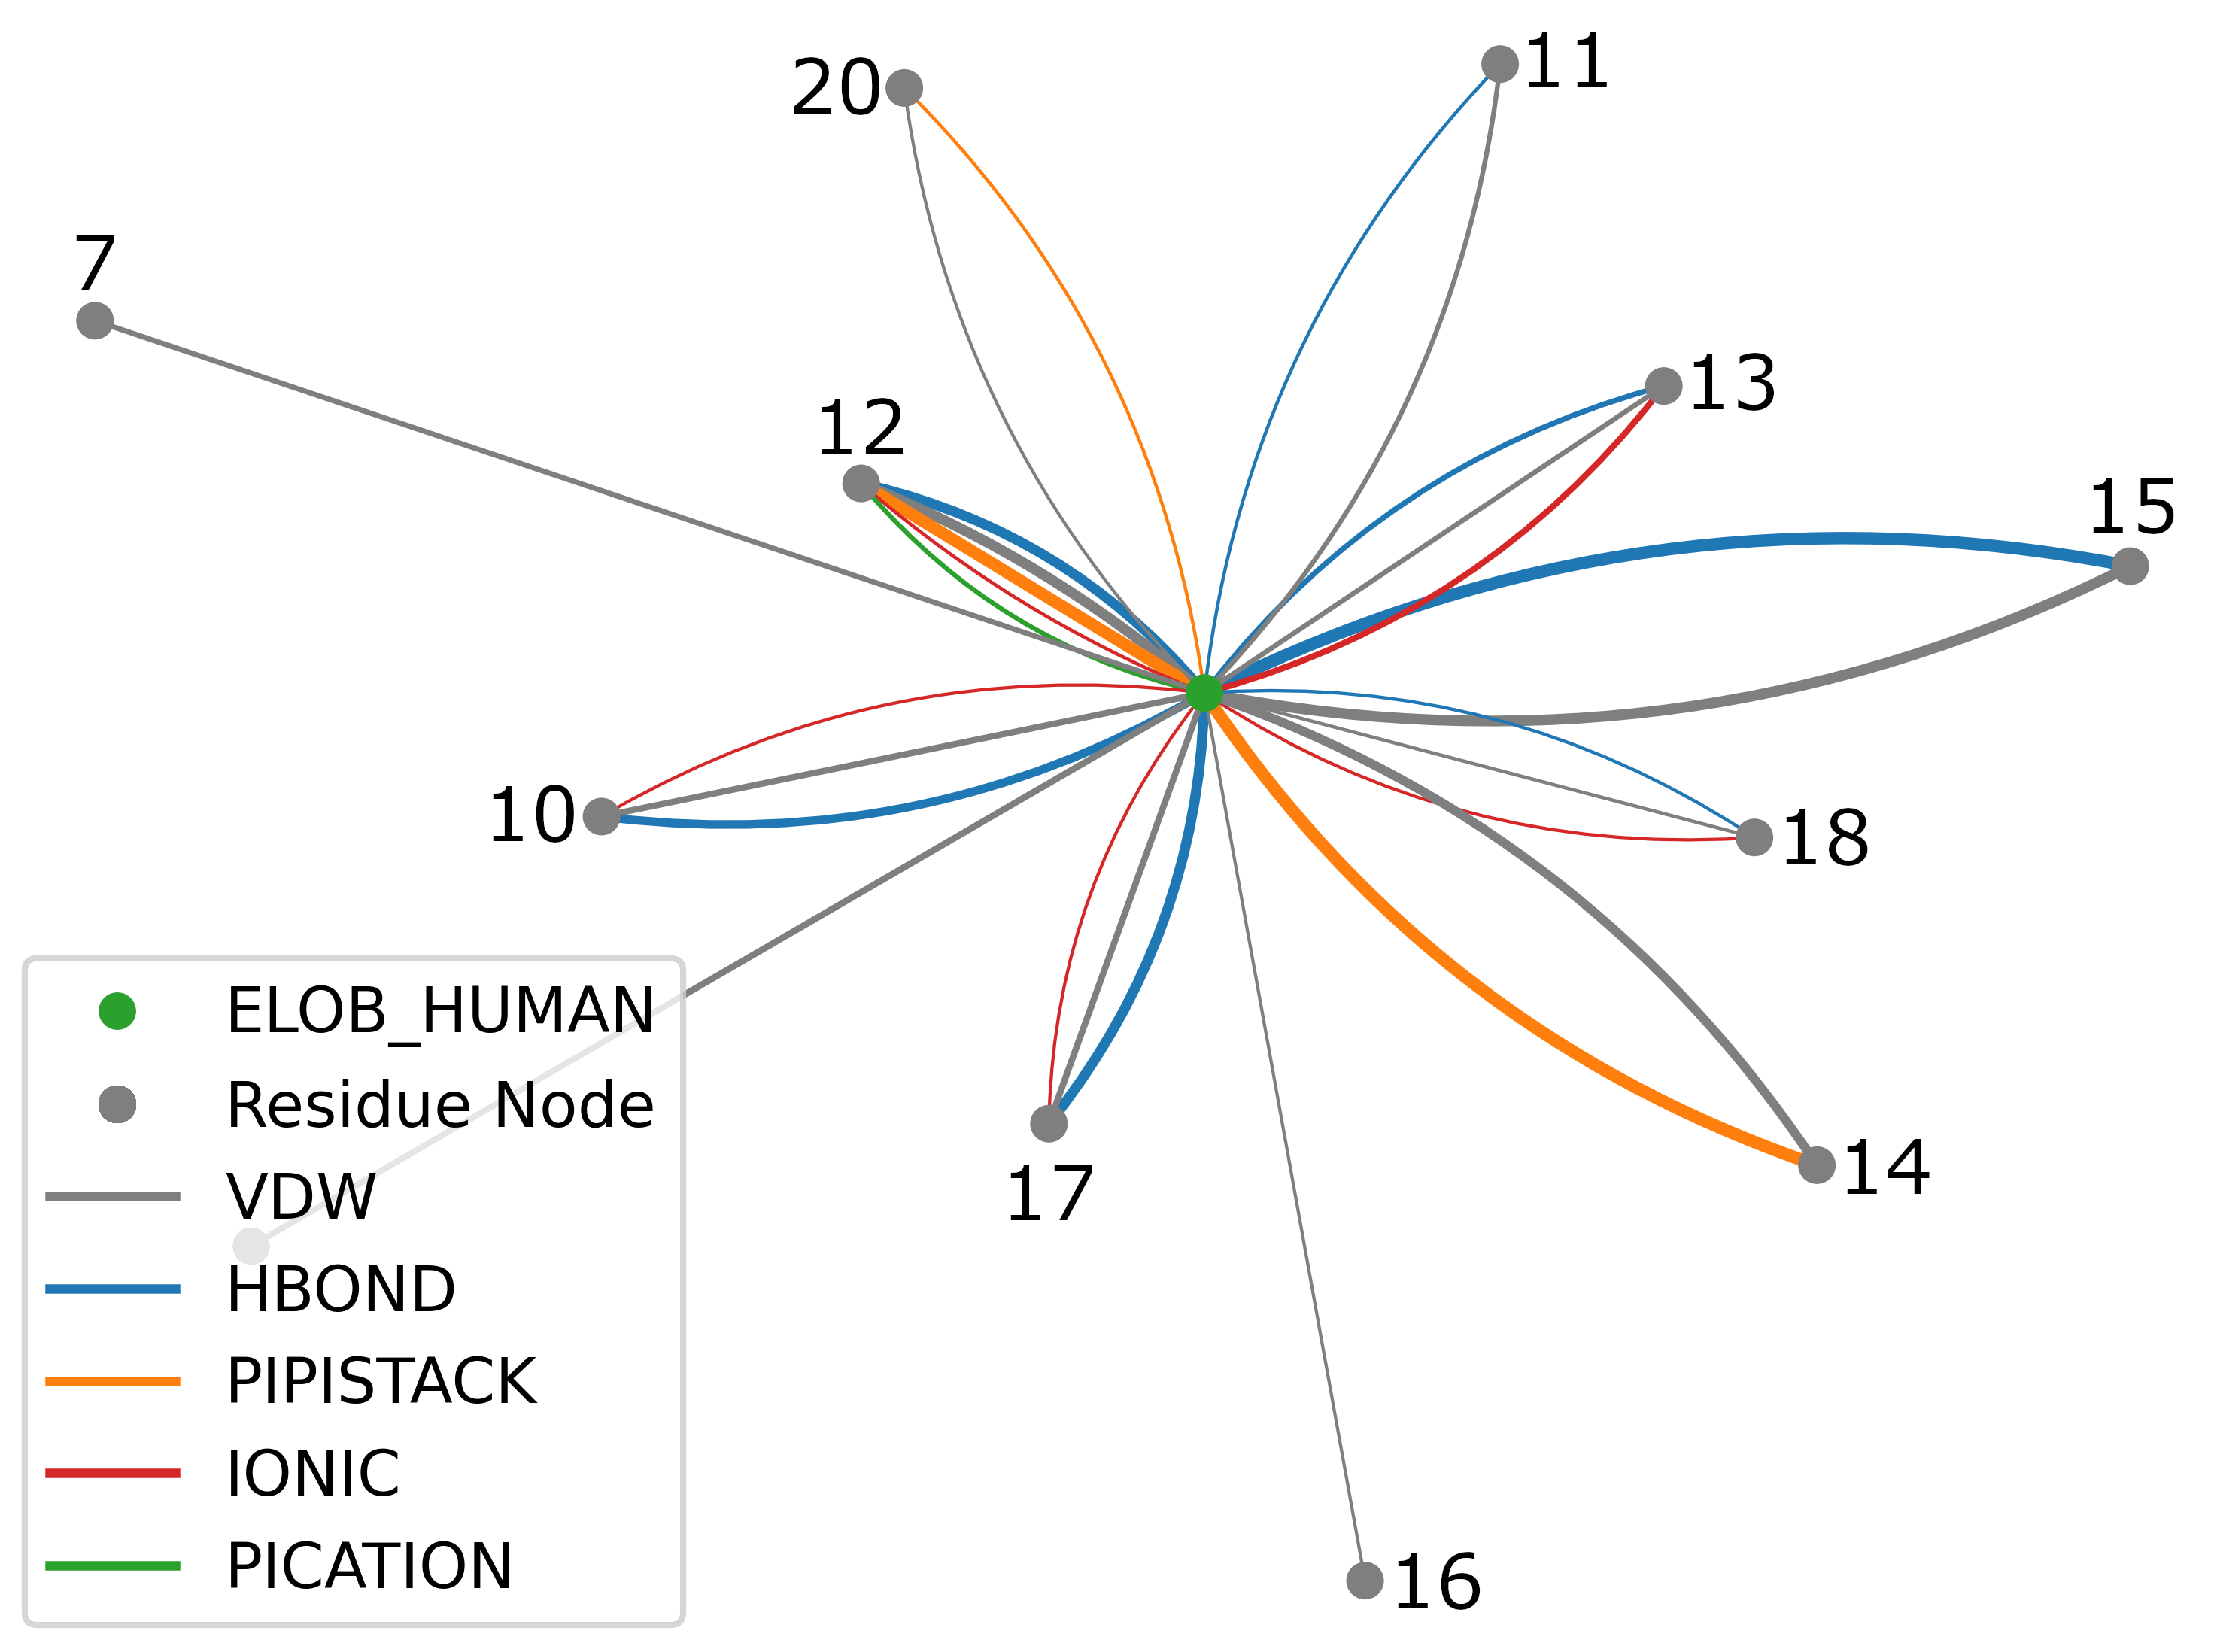
\includegraphics[width=\textwidth]{fig/eloc-bsheet-net.png}
    \caption{Sub-network of hRIN created for studying the inter-chain interaction between ELOC\_HUMAN and ELOB\_HUMAN. Further filtering was performed to consider only residue nodes 11 - 17 corresponding to a $\beta$-sheet comprising the primary stabilizing component of the ELOC - ELOB complex. Where a full network is too large to effectively visualize, this network clearly displays the the degree to which different inter-chain interactions are conserved in the hRIN.}
    \label{fig:eloc-bsheet-net}
\end{figure}

The figure displays noatbly several edges with notably high probability weights, indicating highly conserved interactions in the family. Such interactions can to be intrepreded as highly significant, or key interactions in the protein family. A common inference from such highly conserved interactions with high spesificity are of significant importance to their function. In this case, binding to form a complex with a nother protein chain, which as discussed earlier, is critical for the proteins function.

The network in \ref{fig:eloc-bsheet-net} conveys at a glance information from over 64 structures and 128 distinct ELOC chians. Immediately, we can se that Many residues in ELOC forming hydron bonds and Van Der Waals interactions with ELOB is a significant 

%% Disordered terminus of ELOB held inplace against ELOC mainly by weaker VDW and HYDROGEN BOND forces

%% Getting information about the disorderd tail would best be done with ELOB as the query sequence
% Table for entities present in each homolog structure.


% 2 isoforms
% VHL negatively regulate hypoxia induced products
% What is EL ubiquitin ligase in connection to this context?
%% Substrate recognition
% VHL disease
%Hareditary form of cancer caused by germline mutations
% Highly vascular
% What is angiogenisis - not *not really needed*
% note the interaction of pVHL and HIF-A conservation between species (Maxwell(?)) -- read this on wikipedia

% pVHL ELOC interaction

The binding of pVHL to 
negatively regulates the 
A conserved region on elongin C consisting of residues 17-50 is needed for the binding of Elongin C to pVHL \cite{Ohh1999}.
%Isoforms
%A2 only expressed in the testis

Elongins are a member of the ... superfamily
Elongin A is primarily responsible for nucleotide interaction and transcription function where the other sub units serve regulatory functions.
% Talk about the interactions and the nature of the VHL as a disordered protein
% Describe VHL role in cancer
VHL owes its name with its association with a long known form of cancer inherited cancer - von Hippel-Lindau disease which has come to be associated with with the VHL gene. 
VHL functions as a tumor suppressor and has many known interactions, and though  VHL is not known to have close homologs, it interacts with other genes important for RNA transcription processes [VHLdb][sci-direct]. 
Among it's known interactions is with Elongin C, which participates in in humans is part of the Transcription factor B/SIII complex.
% Possible analysis:
% 1. Run pipeline on ELOC_HUMAN
% Run the pipeline with VHL as the query chain to see if there is conservation / variation of interaction information
We investigate the specificity of interactions between Elongin C and VHL by initiating the HomologyRing pipeline using the Elongin C present in PDB: 


\subsection{DDX}
%%% NEW INTRODUCTION
DEAD-box RNA helicases, or here otherwise referred to as members of the DDX family of proteins, are critical for many processes involving RNA metabolism and are the subject of much research due to their role in the formation of many cancers. They are responsible for ATP-dependent RNA binding and remodeling, with members assuming general and more specialized roles in RNA metabolism including: RNA duplex unwinding, 
We examine hRIN created from a set of human DDX paralogues, to examine key interactions between residues in the family, and compare the results to current literature to illustrate the effectiveness of HomologyRing to identify residues and interactions critically important for the function of a family of proteins. In this case, illustrating its usefulness in studying a verity of studies, including virology, genome protection, and cancer. (big sell)

There are DDX homologs are found in all kingdoms of life including viruses; many organisms having many paralogs. Humans are currently known to have 38 (cite)
DDX proteins are members of the helicase superfamily 2 (SF2). 
Intrensically disordered N- and C- terminal domains exhibit high sequence variability within the family, which may contain sequences responsible for regulation, protein localization, or even additional folded domains. Consequently, the terminal regions will exhibit low conservation of sequence and non-covalent interactions.

The DDX protein will bind to the phosphate backbone of one strand of dimerized RNA. The two recA domains of the DDX proteins contain the substrates that interface with the phosphate backbone of an RNA strand. This substrate is variably conserved, allowing for some members of the DDX family to be more generalists, while others exbibit RNA-sequence specificity (super need a citation for that.) 
ATP binds to a an eponymous D-E-A-D box region of the DDX protein. This refers to a highly conserved Asp-Glu-Ala-Asp motif responsible for ATP binding, mutations of which are known to be highly oncogenic (citation). When bound to an RNA duplex, energy from ATP in complex can be used to introduce a 'kink' in the backbone of one strand in the RNA duplex. The conformal change of the strand induces a local separation of the RNA strands.

%% WHAT WE AIM TO SHOW
In this section, we aim to examine the conservation of \emph{intra-chain} contacts with a family of 37 paralogues and compare conserved interactions with notable conserved structural features characteristic of the family from literature. 

% PROCEDURE
In this section, a hRIN is created from a set of user supplied homologs, which HomologyRing supports. This is in contrast to providing a query and letting HomologyRing do a homology search to select homolog structures from a database. 

To begin creating the custom DDX family, a query was executed agains the UniprotKB database for entries containing the prosite-PS51192 domain wich corresponds to Helicase 1 ATP Binding Domain. Prosite is a curated database of protein families, domains and, functional sites, wich is useful for getting entries for retreiving structures wit a common feature. In this case, we restrict the Uniprot query to results with structures in the PDB and belonging to Homo sapiens. The results were downloaded and furter filtered in python; keeping only resyts that are annotated in UniProt as being transcribed from a DDX gene. This step is necessary as there are a handful of other genes whos gene products exhibit this domain. The resulting collection of Uniprot entries represents 36 human DDX paralogues with 240 corresponding structures in the PDB. These results are further filtered by using pcbecif's CIF parcer python package to create the final protein family, the subject of our analysis by considering the PDB metadata included in the structure files.

%%% BEGIN OLD TEXT %%%
% Needs to be sorted trhough and pick out what is still useful


%% Introduction and biological background
So far we have focused on the homolog use case, which is useful for examining the properties of closely related proteins as measured by sequence similarity. HomologyRing allows the user to provide their own family for which to create an hRIN and perform analysis by giving a list of structures. 
We display this functionality on a family of RNA dependent DEAD-box ATPases (DDXs) paralogs in Humans. 
The analysis of paralogs is 
The family of paralogs has notably lower sequence identity when comapred to common families returned by BLAST homology search with typical parameters.
This family has receives much attention for their essential roll in RNA processing


DDXs are responsible for many different roles involving RNA processing. Primary of which is the unwinding of RNA duplexes in an ATP-dependent mannor. This is crutial in RNA transcriptionm splicing, translation initiation, transport, and degradation.
As such, they are observed in virtually all living organisms. Eukaryotes will often will possess many paralogs of DDX with many becoming highly specillized for spesific process, while others remain serving more general roles in RNA metabolism.

% Introduction
DDX proteins are also called DEAD-box proteins for a higly conserved Asp-Glu-Ala-Asp motif at the RNA substrate interface.
They are responsible for binding and `kinking' RNA in an ATP dependent manner. 
The resulting RNA-peptide complex can either part of an RNA binding portion of a larger protein complex, or be resposible for the local unwinding of double stranded RNA duplexes. 
% Does the DEAD-box always bind to the backbone?
% Talk about conserved DEAD-box site
% conserved ATP binding site
These sites are curutial for the core responsiblies of all members of the DEAD-box family. There are a handful of other conserved motifs including: ...
Additionally the globular core of the DDX proteins are part of the (What is the name of the fold?) and is well conserved. 
In contrast, the N- and C- terminal regions of members are highly variable and spesific to the specialized functions of members.

Some members are generalists , involved in many or critical proliferic RNA matabolisim pathways \todo{such as...}.
Others adopt a more specialaized role.


The roll of DDX proteins as RNA remodelsers make them cridical for virtually all forms of life. However, they have additionally attacted additional attention for their role in cancer \cite{genes12101471}. 
% Elaborate
% Genetic stability for its roll in DNA Repair
% Lift introduction form this article

A great deal of variation is seen within the family to support the specilization of different proteins, but several conserved motifs and domains remain characteristic of the family and well conserved. 
They all share a common helicase domain that constitutes a globular core.
% RecA fold of core associated with helicase domain
% DEAD-BOX
% SAT - substrate binding
% Q motif - ATP binding
% Divergen terminal regions responsible for RNA binding and protein cofactors
% organelle presence and what even is a condensate???

%% PROCEDURE
There are 38 known DDX paralogs in the human proteome \cite{placeholder}. Being paralogues, they are the result of a \emph{gene duplication event}, and have been subject many mutations since allowing for variations in structure and function. The details of this process are provided earlier in \ref{subsec:paralogs} DDX proteins are crutial for virtually all processes involving RNA metabolism \cite{placeholder}. \todo{Better word than matabolism?}. 

In this section, we analize the set of human DDX paralogs to identify 
A set of 38  PDB structures representing DDX paralogues where manually curated. Structures where chosen that have good biological assemblies, meaning most structures where complexes of multiple chains. To initiate the pipeline on a user-defined family, homolog chains to be considered for the analyis must be provided to the HomologyRing tool, and was collected using gene metadata within the collected CIF files. 
The construction of the hRIN via the HomologyRing pipeline works much the same, except the homology search may be skipped given the provided information. 

%% RESULTS
Observe that highly conserved interactions within the family correspond to regions of critical functional importance.

We find that the interactions with the highest conservation score in the family is hydrogen bonds maintaining a local conformation around the DEAD box - which is critical for protein-nucleotide interface and the functioning of all DDX proteins